\documentclass[10pt]{article}
\usepackage[a4paper,margin=1.6cm,top=1.3cm,bottom=1.3cm]{geometry}
\usepackage[T1]{fontenc}
\usepackage{lmodern}
\usepackage{microtype}
\usepackage{booktabs}
\usepackage{graphicx}
\usepackage{enumitem}
\usepackage{xcolor}
\usepackage[colorlinks=true,linkcolor=black,citecolor=black,urlcolor=blue]{hyperref}
\setlist{nosep,leftmargin=1.2em,topsep=1pt}
\setlength{\parindent}{0pt}
\setlength{\parskip}{3pt}
\pagestyle{empty}
\newcommand{\head}[1]{\par\smallskip{\large\bfseries #1}\par}
\newcommand{\sect}[1]{\par\smallskip{\bfseries\color{black!80} #1}\par}

\begin{document}
\head{Idea 8 PoC --- Do LLM forecasters inherit the gambler's fallacy?}
\textit{Proof of concept, October 2026. Code: \texttt{run.py} (model alias as argument) and \texttt{compare.py}.}

\sect{Question and design}
LLMs are increasingly used as forecasters and as proxies for human expectations (Kim, Muhn and Nikolaev, 2024;
Bybee, 2023). Do they show the gambler's fallacy, expecting a streak of earnings increases to end? Or do they show
the hot hand, or neither? Each case is an \emph{anonymised} history of 12 standalone quarterly EPS: oldest first,
labelled only by fiscal quarter, rescaled by a random firm-specific constant, and without names or dates, so the
model cannot recognise the firm or look ahead. The model returns a point forecast for the next quarter and
$p_{up}$, the probability that it beats the same quarter a year earlier. There are 320 cases (FY2012--2019),
stratified with 40 per bucket by the current streak of year-on-year EPS changes ($-4^+$ to $+4^+$). Models are
Claude Haiku and Claude Sonnet, called headlessly through the local \texttt{claude} CLI (20 series per call, no tools;
total cost \$3.65). Realised frequencies and XGBoost are computed on all 52{,}705 eligible cases. Under the gambler's
fallacy, $p_{up}$ would \emph{fall} along up-streaks; under the hot hand, it would rise faster than outcomes do.

\begin{center}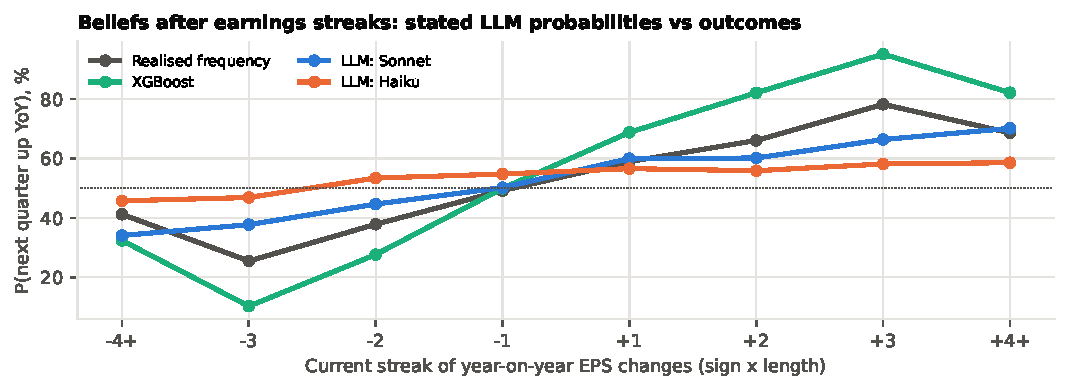
\includegraphics[width=0.97\textwidth]{results/fig_compare.pdf}\end{center}

\begin{center}\small
\begin{tabular}{lcccc}
\toprule
 & Slope of $p_{up}$ on & Slope of $p_{up}$ on & Median abs.\ error & Direction\\
 & up-streak length & down-streak length & (scaled units) & accuracy\\
\midrule
LLM: Haiku & 0.008 (0.5) & $-0.034$ ($-1.9$) & 48.6 & 60.3\%\\
LLM: Sonnet & 0.037 (3.9) & $-0.055$ ($-4.9$) & 36.4 & 68.8\%\\
Realised outcome & 0.065 (2.0) & $-0.060$ ($-1.7$) & -- & --\\
XGBoost (share of forecasts up) & 0.047 (1.6) & $-0.095$ ($-2.8$) & 39.8 & 71.6\%\\
Seasonal random walk & -- & -- & 45.1 & --\\
\bottomrule
\end{tabular}\\[2pt]
{\footnotesize Slopes per additional quarter of streak ($t$, clustered by firm), on the 320 LLM cases.
Brier score of $p_{up}$: Haiku 0.257, Sonnet 0.207.}
\end{center}

\sect{Findings}
\begin{itemize}
\item \textbf{No gambler's fallacy in either model.} Neither model lowers its probability of an increase as an
  up-streak lengthens. Year-on-year EPS changes are persistent in the data, and both models lean, correctly, toward
  continuation.
\item \textbf{The smaller model is conservative, not biased.} Haiku's probabilities hug 50\% (46--59\%) and barely
  respond to streaks: an underreaction pattern, like sticky expectations. Sonnet's beliefs move with the streak at
  about two-thirds of the realised slope, with no overreaction.
\item \textbf{A capable LLM is a competitive forecaster on anonymised data.} Sonnet's point forecasts have a lower
  median error than XGBoost and the SRW on these cases. Its directional accuracy is slightly below XGBoost's (68.8\%
  vs 71.6\%).
\end{itemize}

\sect{Assessment and next steps}
The headline hypothesis is rejected, but the PoC delivers a clean, leakage-robust protocol. It also yields an
interesting dose-response: underreaction shrinks with model capability. Next steps: (i) scale to several thousand
cases and more models, including open-weight ones; (ii) elicit beliefs in the \emph{surprise} domain the paper uses
(``will EPS beat the forecast?''), where the fallacy is defined; (iii) prompt variants that add a human-style
narrative (``five quarters of growth in a row'') to test framing; (iv) check whether LLM-implied surprises explain
announcement returns better than statistical ones, as a ``synthetic retail investor''. Fast-moving field: best
targeted at a top field journal quickly.
\end{document}
